\documentclass[]{politex}
% ========== Opções ==========
% pnumromarab - Numeração de páginas usando algarismos romanos na parte pré-textual e arábicos na parte textual
% abnttoc - Forçar paginação no sumário conforme ABNT (inclui "p." na frente das páginas)
% normalnum - Numeração contínua de figuras e tabelas 
%	(caso contrário, a numeração é reiniciada a cada capítulo)
% draftprint - Ajusta as margens para impressão de rascunhos
%	(reduz a margem interna)
% twosideprint - Ajusta as margens para impressão frente e verso
% capsec - Forçar letras maiúsculas no título das seções
% espacosimples - Documento usando espaçamento simples
% espacoduplo - Documento usando espaçamento duplo
%	(o padrão é usar espaçamento 1.5)
% times - Tenta usar a fonte Times New Roman para o corpo do texto
% noindentfirst - Não indenta o primeiro parágrafo dos capítulos/seções


% ========== Packages ==========
\usepackage[utf8]{inputenc}
\usepackage{amsmath,amsthm,amsfonts,amssymb}
\usepackage{graphicx,cite,enumerate}


% ========== Language options ==========
\usepackage[brazil]{babel}
%\usepackage[english]{babel}


% ========== ABNT (requer ABNTeX 2) ==========
%	http://www.ctan.org/tex-archive/macros/latex/contrib/abntex2
%\usepackage[num]{abntex2cite}

% Forçar o abntex2 a usar [ ] nas referências ao invés de ( )
%\citebrackets{[}{]}


% ========== Lorem ipsum ==========
\usepackage{blindtext}



% ========== Opções do documento ==========
% Título
\titulo{Simulação dinâmica e validação experimental de técnicas de controle para manipuladores paralelos}

% Autor
\autor{André Garnier Coutinho}

% Para múltiplos autores (TCC)
%\autor{Nome Sobrenome\\%
%		Nome Sobrenome\\%
%		Nome Sobrenome}

% Orientador / Coorientador
\orientador{Prof. Dr. Tarcisio Antonio Hess Coelho}
%\coorientador{Nome do coorientador (opcional)}

% Tipo de documento
%\tcc{Eletricista com ênfase em Sistemas Eletrônicos}
%\dissertacao{Engenharia Elétrica}
\teseDOC{Engenharia Mecânica}
%\teseLD
%\memorialLD

% Departamento e área de concentração
\departamento{PMR – Eng. Mecatrônica e de Sistemas Mecânicos}
\areaConcentracao{Engenharia Mecânica de Projeto e Fabricação}

% Local
\local{São Paulo}

% Ano
\data{2019}




\begin{document}
% ========== Capa e folhas de rosto ==========
\capa
\falsafolhaderosto
\folhaderosto


% ========== Folha de assinaturas (opcional) ==========
\begin{folhadeaprovacao}
	\assinatura{Prof. Dr. Tarcisio Antonio Hess Coelho}
	\assinatura{Prof. Dr. Renato Maia Matarazzo Orsino}
	\assinatura{Profª. Dra. Maira Martins da Silva}
	\assinatura{Prof. Dr. Bruno Augusto Angélico}
	\assinatura{Prof. Dr. Diego Colón}
\end{folhadeaprovacao}


% ========== Ficha catalográfica ==========
% Fazer solicitação no site:
%	http://www.poli.usp.br/en/bibliotecas/servicos/catalogacao-na-publicacao.html


% ========== Dedicatória (opcional) ==========
%\dedicatoria{Dedicatória}


% ========== Agradecimentos ==========
\begin{agradecimentos}

Gostaria de agradecer a todos que sempre me apoiaram e ajudaram a perseguir o meu sonho de me tornar Doutor em Engenharia Mecânica pela Escola Politécnia da USP. Não tenho palavras para descrever o que significa para mim poder estar contribuindo ativamente na exploração das fronteiras do conhecimento.

Dentre as várias pessoas que sempre estiveram ao lado nesta jornada, gostaria de destacar o meu orientador e amigo Prof. Dr. Tarcisio Antonio Hess Coelho, o qual sempre esteve ao meu lado desde o início da jornada no meio acadêmico, sempre sendo super solícito, me apoiando, e me orientando da melhor maneira possível; meu grande amigo Prof. Dr. Renato Maia Matarazzo Orsino, o qual me introduziu e ensinou o que há de mais sofisticado e eficiente na parte de modelagem de sistemas multicorpos, um conhecimento fundamental para o desenvolvimento desta tese, também sempre sendo extremamente solícito e me ajudando sempre que podia; aos grandes amigos Engª. Juliana Martins de Oliveira Fuess e Eng. Victor Pacheco Bartholomeu, os quais participaram ativamente e possibilitaram o desenvolvimento do protótipo de manipulador paralelo que possibilitou adicionar um caráter experimental na tese desenvolvida; à minha namorada Adriana Marques Cavalcanti, a qual está há mais de 12 anos ao meu lado, sempre me apoiando em todos os momentos e me inspirando a ser cada vez mais uma pessoa melhor; e aos meus pais Antonio Valdec Martins Coutinho e Taïs Borges Garnier, e avó Maria Luiza Borges Garnier, os quais estão sempre se preocuparam muito comigo, sempre me apoiando e ajudando de todas as maneiras.

Por último, mas não menos importante, além dessas pessoas incríveis que tive a oportunidade de conhecer em minha vida, gostaria de destacar meu agradecimento a outras três pessoas maravilhosas que conheci há pouco tempo, que mudaram minha vida, e que tornaram possível a conclusão desta tese de doutorado: minha psicóloga Dra. Ana Maria Canzonieri, minha psiquiatra Dra. Letícia Pacheco Lessa, e minha professora de yoga Alessandra Dotto.

Muito obrigado a todos, sem vocês nada disso seria possível.

\end{agradecimentos}


% ========== Epígrafe (opcional) ==========
\epigrafe{%
	\emph{`` `Nesta direção', disse o Gato, girando a pata direita, `mora um Chapeleiro. E nesta direção', apontando com a pata esquerda, `mora uma Lebre de Março. Visite quem você quiser, são ambos loucos.' \\
	`Mas eu não ando com loucos', observou Alice. \\
	`Oh, você não tem como evitar', disse o Gato, `somos todos loucos por aqui. Eu sou louco. Você é louca'. \\
	`Como é que você sabe que eu sou louca?', disse Alice. \\
	`Você deve ser', disse o Gato, `Senão não teria vindo para cá.' ''}
	\begin{flushright}
		-{}- Lewis Carroll
	\end{flushright}
}


% ========== Resumo ==========
\begin{resumo}
Para realizar o projeto de um sistema de controle, em geral, \'e necess\'ario primeiramente de um modelo da planta a ser controlada. O grau de fidelidade do modelo da planta, dentro das condi\c{c}\~oes de opera\c{c}\~ao desejadas do sistema, influi diretamente no desempenho do sistema em malha fechada que o projeto do controlador pode oferecer. Quanto mais rico for o modelo, mais f\'acil de atingir requisitos de desempenho mais elevados (menor tempo de resposta e menor sobressinal, por exemplo) garantindo a estabilidade do sistema.

Utilizando os m\'etodos tradicionais de modelagem de Sistemas Mec\^anicos Multicorpos, \'e dif\'icil e trabalhoso de se obter modelos de sistemas complexos, como mecanismos paralelos. Para contornar esse problema, \'e comum desprezar alguns efeitos de acoplamentos inerciais, simplificando o processo de modelagem. Por\'em, essa estrat\'egia gera modelos mais pobres, o que ir\'a limitar o desempenho que o sistema poder\'a atingir quando for feito o projeto do sistema de controle.

A solu\c{c}\~ao proposta para ser poss\'ivel aumentar o desempenho, garantindo a robustez, de um sistema de controle de mecanismos paralelos \'e a utiliza\c{c}\~ao dos novos m\'etodos e estratégias de modelagem din\^amica desenvolvidos pelo grupo de pesquisa do Prof. Doutor Tarcisio Antonio Hess Coelho, os quais s\~ao adequados para incluir todos os efeitos da din\^amica de corpos r\'igidos, independentemente da complexidade do sistema.

A presente tese visa desenvolver um algoritmo de modelagem que inclua todos os efeitos da din\^amica de corpos r\'igidos para realizar a modelagem din\^amica de mecanismos paralelos (baseado na metodologia Orsino), desenvolver uma metodologias de projeto de controle robusto para mecanismos paralelos tradicionais e mecanismos com atua\c{c}\~ao redundante, e realizar simulações e valida\c{c}\~oes experimentais das leis de controle sintetizadas pela metodologia proposta.
%
\\[3\baselineskip]
%
\textbf{Palavras-Chave} -- Mecanismos paralelos, Robótica, Modelagem Dinâmica , Controle, Controle não linear.
\end{resumo}


% ========== Abstract ==========
\begin{abstract}
Abstract...
%
\\[3\baselineskip]
%
\textbf{Keywords} -- Word, Word, Word, Word, Word.
\end{abstract}


% ========== Listas (opcional) ==========
\listadefiguras
\listadetabelas

% ========== Sumário ==========
\sumario



% ========== Elementos textuais ==========

\part{Introdução}
	
\chapter{Introdução}
\capepigrafe[0.5\textwidth]{``Frase espirituosa de um autor famoso''}{Autor famoso}

Os mecanismos de arquitetura paralela são amplamente utilizados em simuladores de voo, simuladores automobilisticos, e tarefas de {\em pick-and-place}. Além disso, também são empregados em sistemas de posicionamento, sistemas de medição, máquinas de usinagem, entre outras tarefas. 

Há uma série de vantagens em utilizar mecanismos paralelos no lugar dos tradicionais seriais. Dentre elas podemos citar sua grande capacidade de carga, alta precisão de posicionamento, alta rigidez estrutural, e uma redução significativa na inércia \cite{Cheng, Khalil, Merlet2002, Tsai}. Outra característica marcante desse tipo de arquitetura são as altas velocidades e acelerações atingidas, as quais superam muito os valores máximos atingidos utilizando arquitetura serial. Grande parte dessas vantagens se devem à possibilidade de instalação de todos os motores na base imóvel do mecanismo. Como desvantagens podemos citar o menor espaço de trabalho e modelo dinâmico muito mais complexo e de difícil obtenção \cite{Rynaldo, Merlet2002}.
%As maiores vantagens em utilizar mecanismos paralelos no lugar dos tradicionais mecanismos seriais são sua grande capacidade de carga, alta precisão de posicionamento do efetuador, alta rigidez estrutural, e uma redução significativa na inércia \cite{Merlet2002, Khalil, Tsai, Cheng}. Outra característica marcante desse tipo de arquitetura são as altas velocidades e acelerações atingidas, as quais superam muito os valores máximos atingidos utilizando arquitetura serial. Grande parte dessas vantagens se devem à possibilidade de ter todos os motores localizados na base. Como desvantagens podemos citar o menor espaço de trabalho e modelo dinâmico muito mais complexo e difícil de se obter \cite{Merlet2002, Rynaldo}.

\begin{figure}[h!]
	\centering
	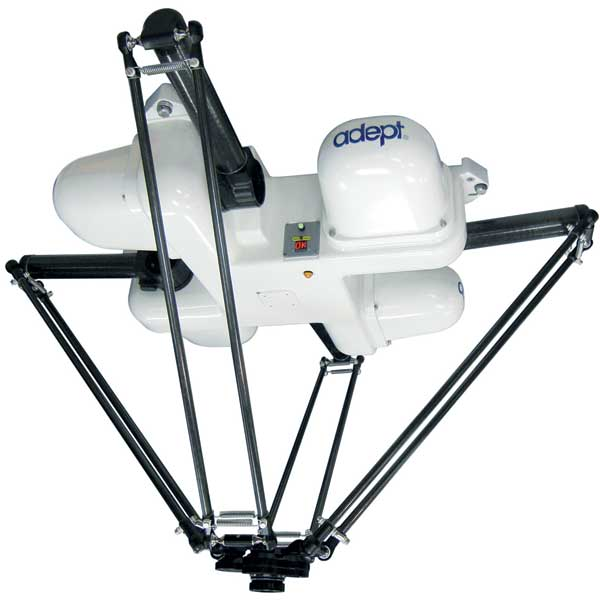
\includegraphics[scale=0.17]{../figures/theadeptquat.jpg}  
	\caption{Robô industrial Adept Quattro}
	\label{fig:Mecanismo}
\end{figure}

Levando-se em conta esta dificuldade de obtenção e a complexidade inerente do modelo dinâmico, o controle de mecanismos de arquitetura paralela é uma tarefa desafiadora. A utilização de modelos dinâmicos simplificados limita o desempenho do projeto de controladores baseados no modelo. Porém, mesmo na hipótese do modelo dinâmico completo estar disponível, o emprego de técnicas de controle não linear pode acarretar um custo  computacional muito elevado \cite{Craig, Slotini, Zubizarreta}. Este paradigma, aliado à falta de estratégias de controle apropriadas para esse tipo de mecanismos, resulta na exploração insatisfatória dos potenciais promissores de tais máquinas, como resposta dinâmica rápida e alta precisão \cite{Abdellatif}. Além disso, observa-se na literatura a escassez de trabalhos publicados com comprovação experimental de técnicas de controle aplicáveis a mecanismos paralelos \cite{Rynaldo}.
	
    Uma alternativa para a superação desta dificuldade seria a combinação de técnicas de controle não linear robusto (por exemplo, controle por modos deslizantes \cite{Slotini, Utkin}) com modelos dinâmicos completos de mecanismos paralelos, desenvolvidos a partir de novas metodologias de modelagem de sistemas multicorpos \cite{22orsino, Orsino2013, 23orsino, 21orsino}. Com esta estratégia, torna-se possível sintetizar leis de controle de alto desempenho e custo computacional mais adequado, viabilizando a exploração do potencial promissor dos mecanismos paralelos.

%OBJETIVOS E JUSTIFICATIVAS--------------------------------------------
\section{Objetivos}\label{objetivos}


Os principais objetivos da tese s\~ao:
\begin{itemize}
\item Desenvolvimento de um algoritmo gerador de modelos dinâmicos completos de mecanismos paralelos, de forma implícita. Será utilizada uma metodologia baseada no método Orsino de acoplamento de subsistemas multicorpos \cite{23orsino}.


\item Elabora\c{c}\~ao de metodologias de projeto de controlador n\~ao linear robusto, de alto desempenho, aplicável a  mecanismos de arquitetura paralela. Para tanto, serão consideradas as incertezas param\'etricas e a possibilidade de atua\c{c}\~ao redundante \cite{Cheng},  além de estratégias para a síntese de leis de controle com custo computacional consideralvemente menor do que as tradicionais, que empregam o Controle por Torque Computado \cite{Craig, Zubizarreta}.

\item Realizar a modelagem cinemática e dinâmica dos mecanismos 5R \cite{22orsino} e 2\underline{R}SU+\underline{P}PaP \cite{Rynaldo, Kumazawa}, utilizando o algoritmo de modelagem desenvolvido.

\item Realizar o projeto de um controlador de trajetória para os mecanismos escolhidos, utilizando a metodologia de projeto de controle proposta.

\item Realizar simula\c{c}\~oes dinâmicas utilizando as leis de controle sintetizadas.

\item Realizar a validação experimental dos controladores projetados no protótipo dos mecanismos 5R, o qual se encontra no laboratório de mecanismos da EPUSP.
\end{itemize}

É importante ressaltar que os 5 primeiros objetivos citados já foram parcialmente alcançados e que a arquitetura paralela 2\underline{R}SU+\underline{P}PaP foi desenvolvida pelo grupo de pesquisa do Prof. Dr. Tarcio Antonio Hess Coelho, havendo ainda poucos estudos na literatura sobre ela. %Sendo assim, pode-se afirmar que simulações dinâmicas e validações experimentais de leis de controle não linear robusto neste mecanismo tem caráter inédito.

%SOBRE A ORGANIZAÇÃO DO TEXTO--------------------------------------------
\section{Sobre a organização do texto}\label{organizacao}

O capítulo 2 apresenta a revisão da Literatura sobre o assunto, sendo que a metodologia da
pesquisa é descrita no capítulo 3. A seguir, os capítulos 4 e 5 abordam a modelagem dinâmica
de manipuladores seriais e paralelos, respectivamente. Com relação ao projeto dos controlado-
res, este assunto é elaborado no capítulo 6. No capítulo 7 são apresentados os resultados mais
relevantes desta Tese, além da pertinente discussão. Por fim, no capítulo 8, apresentam-se as
principais conclusões da Tese e os temas sugeridos para pesquisa futura.

%REVISAO--------------------------------------------------------------------
\chapter{Revisão da literatura}\label{revision}

Esta seção é dedicada à revisão da literatura de técnicas de controle de posição aplicadas a mecanismos paralelos. \\

Existem diversas técnicas propostas pela literatura para realizar o controle de mecanismos paralelos. Dentre elas, podemos destacar:

\begin{itemize}
\item Controle PID
\item Controle por Torque Computado (CTC)
\item Controle por Torque Computado com pré-alimentação (CTCp)
\item Controle por Torque Computado Estendido (CTCe)
\item Controle Preditivo Baseado em Modelo (CPM)
\item Controle Adaptativo
\item Controle por Modos Deslizantes (CMD)
\end{itemize}

A técnica mais simples consiste na utilização de malhas do tipo PID, controlando cada junta ativa de maneira independente, considerando a dinâmica do mecanismo como distúrbios de controle. Essa técnica é caracterizada por sua facilidade de projeto e implementação, tanto em hardware quanto em software, além de exibir um desempenho satisfatório para movimento lento. Porém, essa técnica não se mostra adequada para a realização de trajetórias em altas velocidades e/ou acelerações \cite{Honegger, Zubizarreta}.

Uma das técnicas de controle mais exploradas na literatura é o Controle por Torque Computado (CTC). Basicamente, é uma técnica de controle não linear, mais conhecida como linearização pela realimentação, aplicada a sistemas mecânicos. A técnica consiste na utilização de duas malhas de controle, uma malha que realiza o desacoplamento do sistema e a compensação das não linearidades, e outra malha composta por PIDs independentes \cite{Craig}. Como resultado, alcança-se um desempenho  superior  àquele obtido utilizando simples PIDs, permitindo inclusive a realização de trajetórias precisas em altas velocidades e/ou acelerações. No entanto, seu desempenho poderá ser limitado pela qualidade/fidelidade do modelo dinâmico utilizado para a compensação das não linearidades \cite{SlotiniSMC}. Sua implementação também é mais complexa, visto que é necessário calcular o modelo dinâmico inverso em tempo real, o que também aumenta consideravelmente seu custo computacional. Além disso, a técnica é sensível a incertezas estruturadas (paramétricas) e não estruturadas (dinâmicas não modeladas). Como exemplos de utilização do CTC, podem ser citados os trabalhos de Cheng at al. \cite{Cheng}, Li e Wu \cite{Li}, Li e Fu \cite{Li2}, Shang at al. \cite{Shang} e Yen at al. \cite{Yen}.

\begin{figure}[h]
	\centering
	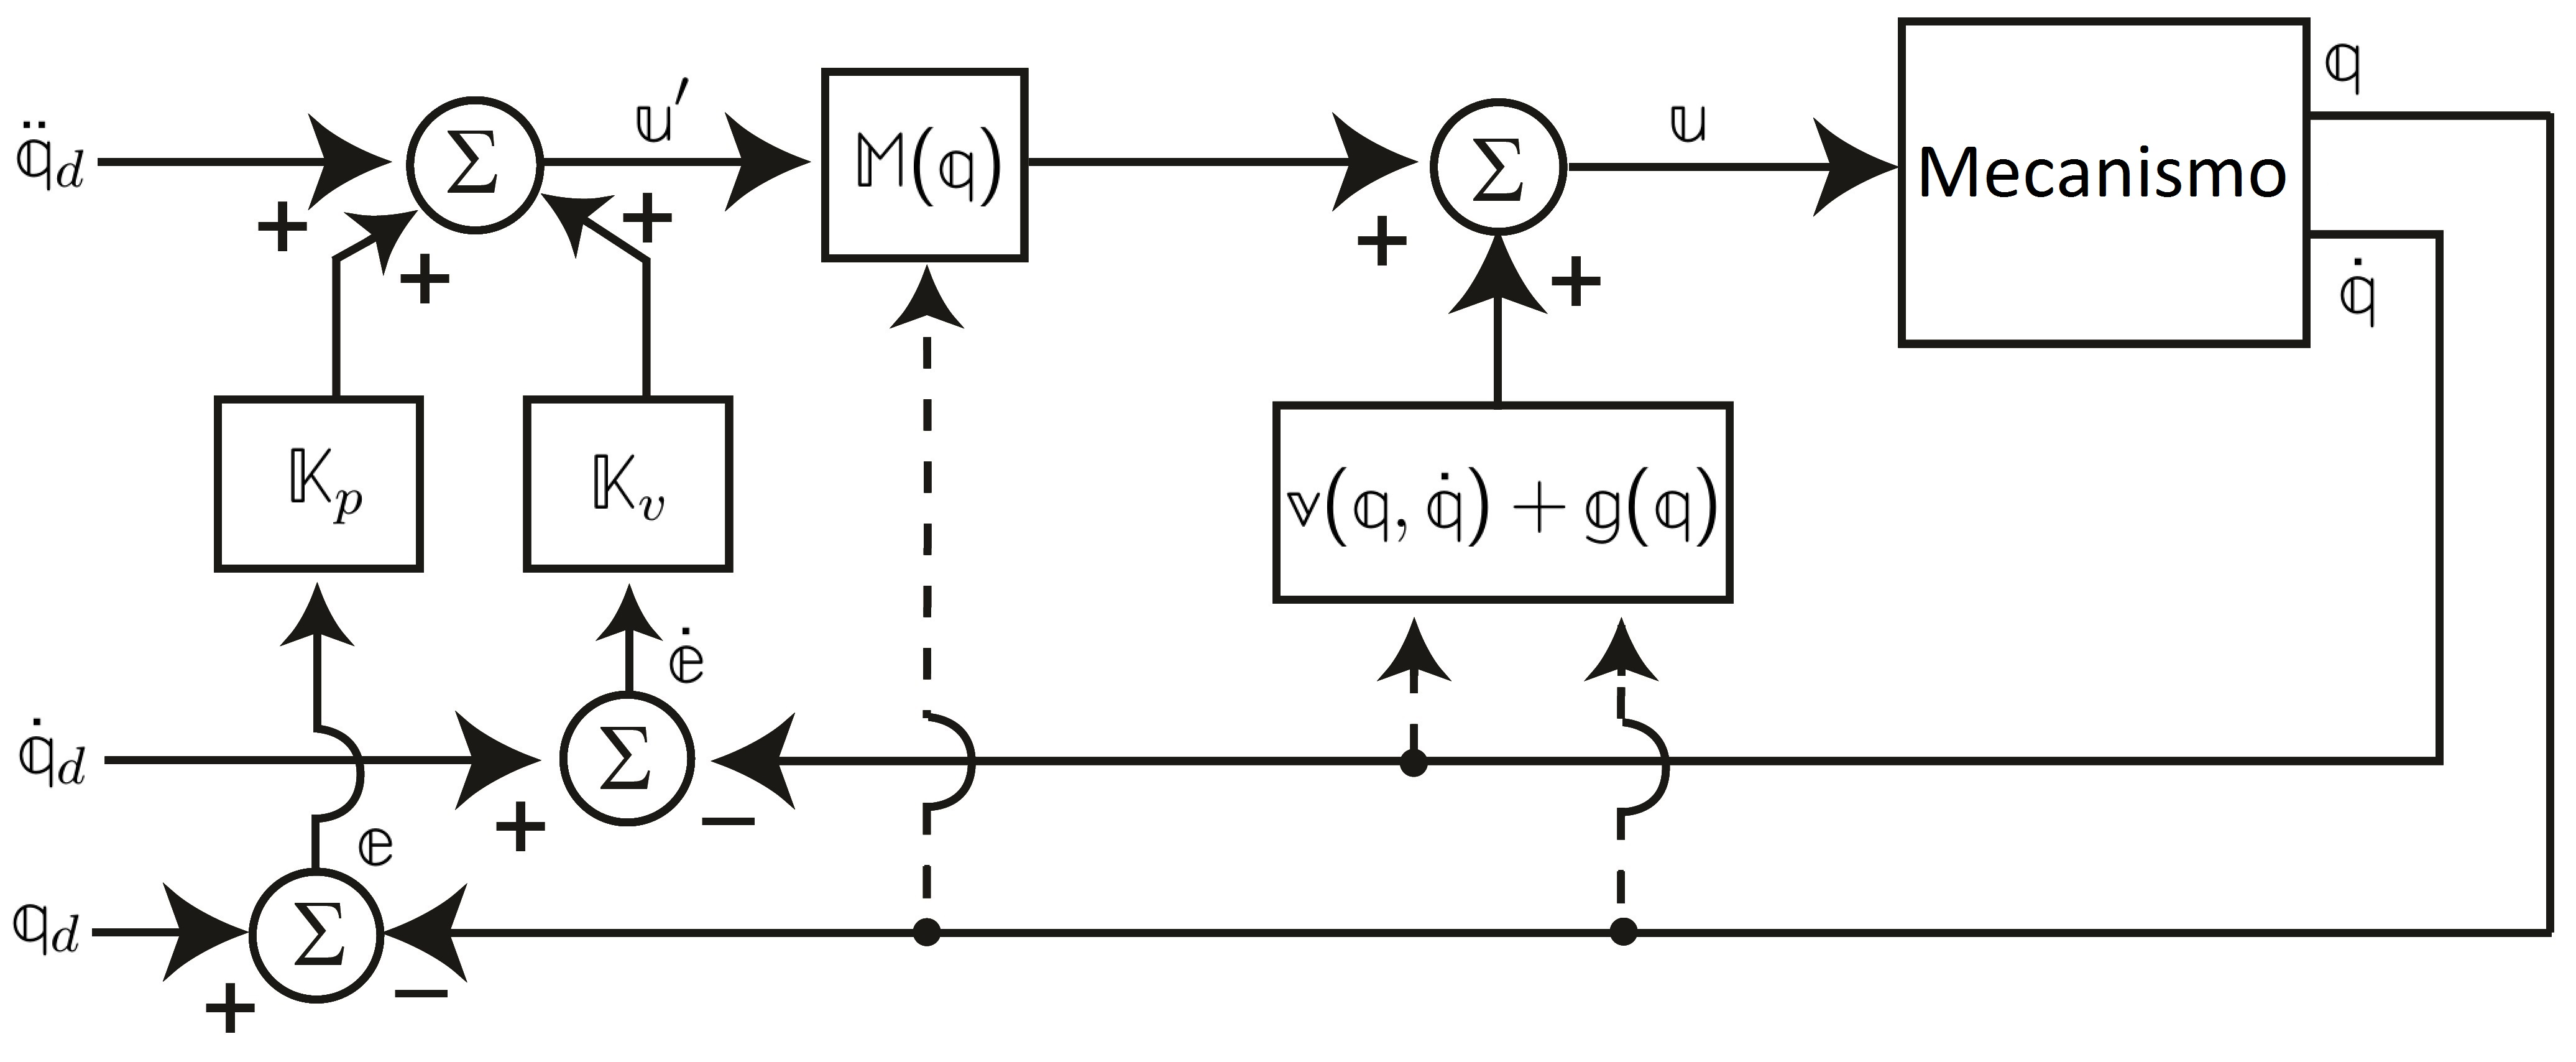
\includegraphics[scale=0.385]{../figures/CTC.jpg}  
	\caption{Malha de CTC (Adaptado de \cite{Craig})}
	\label{fig:CTC}
\end{figure}

Visando a redução do custo computacional associado ao cálculo do modelo dinâmico em tempo real, alguns autores propõe a utilização do CTC com pré-alimentação (CTCp) \cite{Khalil, Siciliano, Spong}. Essa técnica é similar ao CTC, com a diferença de que a compensação das não linearidades é feita por pré-alimentação e não mais por realimentação.  Consequentemente, realiza-se o cálculo do modelo dinâmico previamente, diminuindo o custo computacional.

De fato, Codourey \cite{Codourey} obteve uma redução de 600\% no erro de posição utilizando o CTCp em um ensaio experimental com o robô DELTA, ao substituir os PDs originais. Na simulação do controle de um mecanismo 6-UPS, Wang et al. \cite{Wang} utilizaram em cascata controladores lineares de posição, velocidade e corrente em cada junta ativa, além de  uma compensação dinâmica por pré-alimentação dos distúrbios de torque.

\begin{figure}[h]
	\centering
	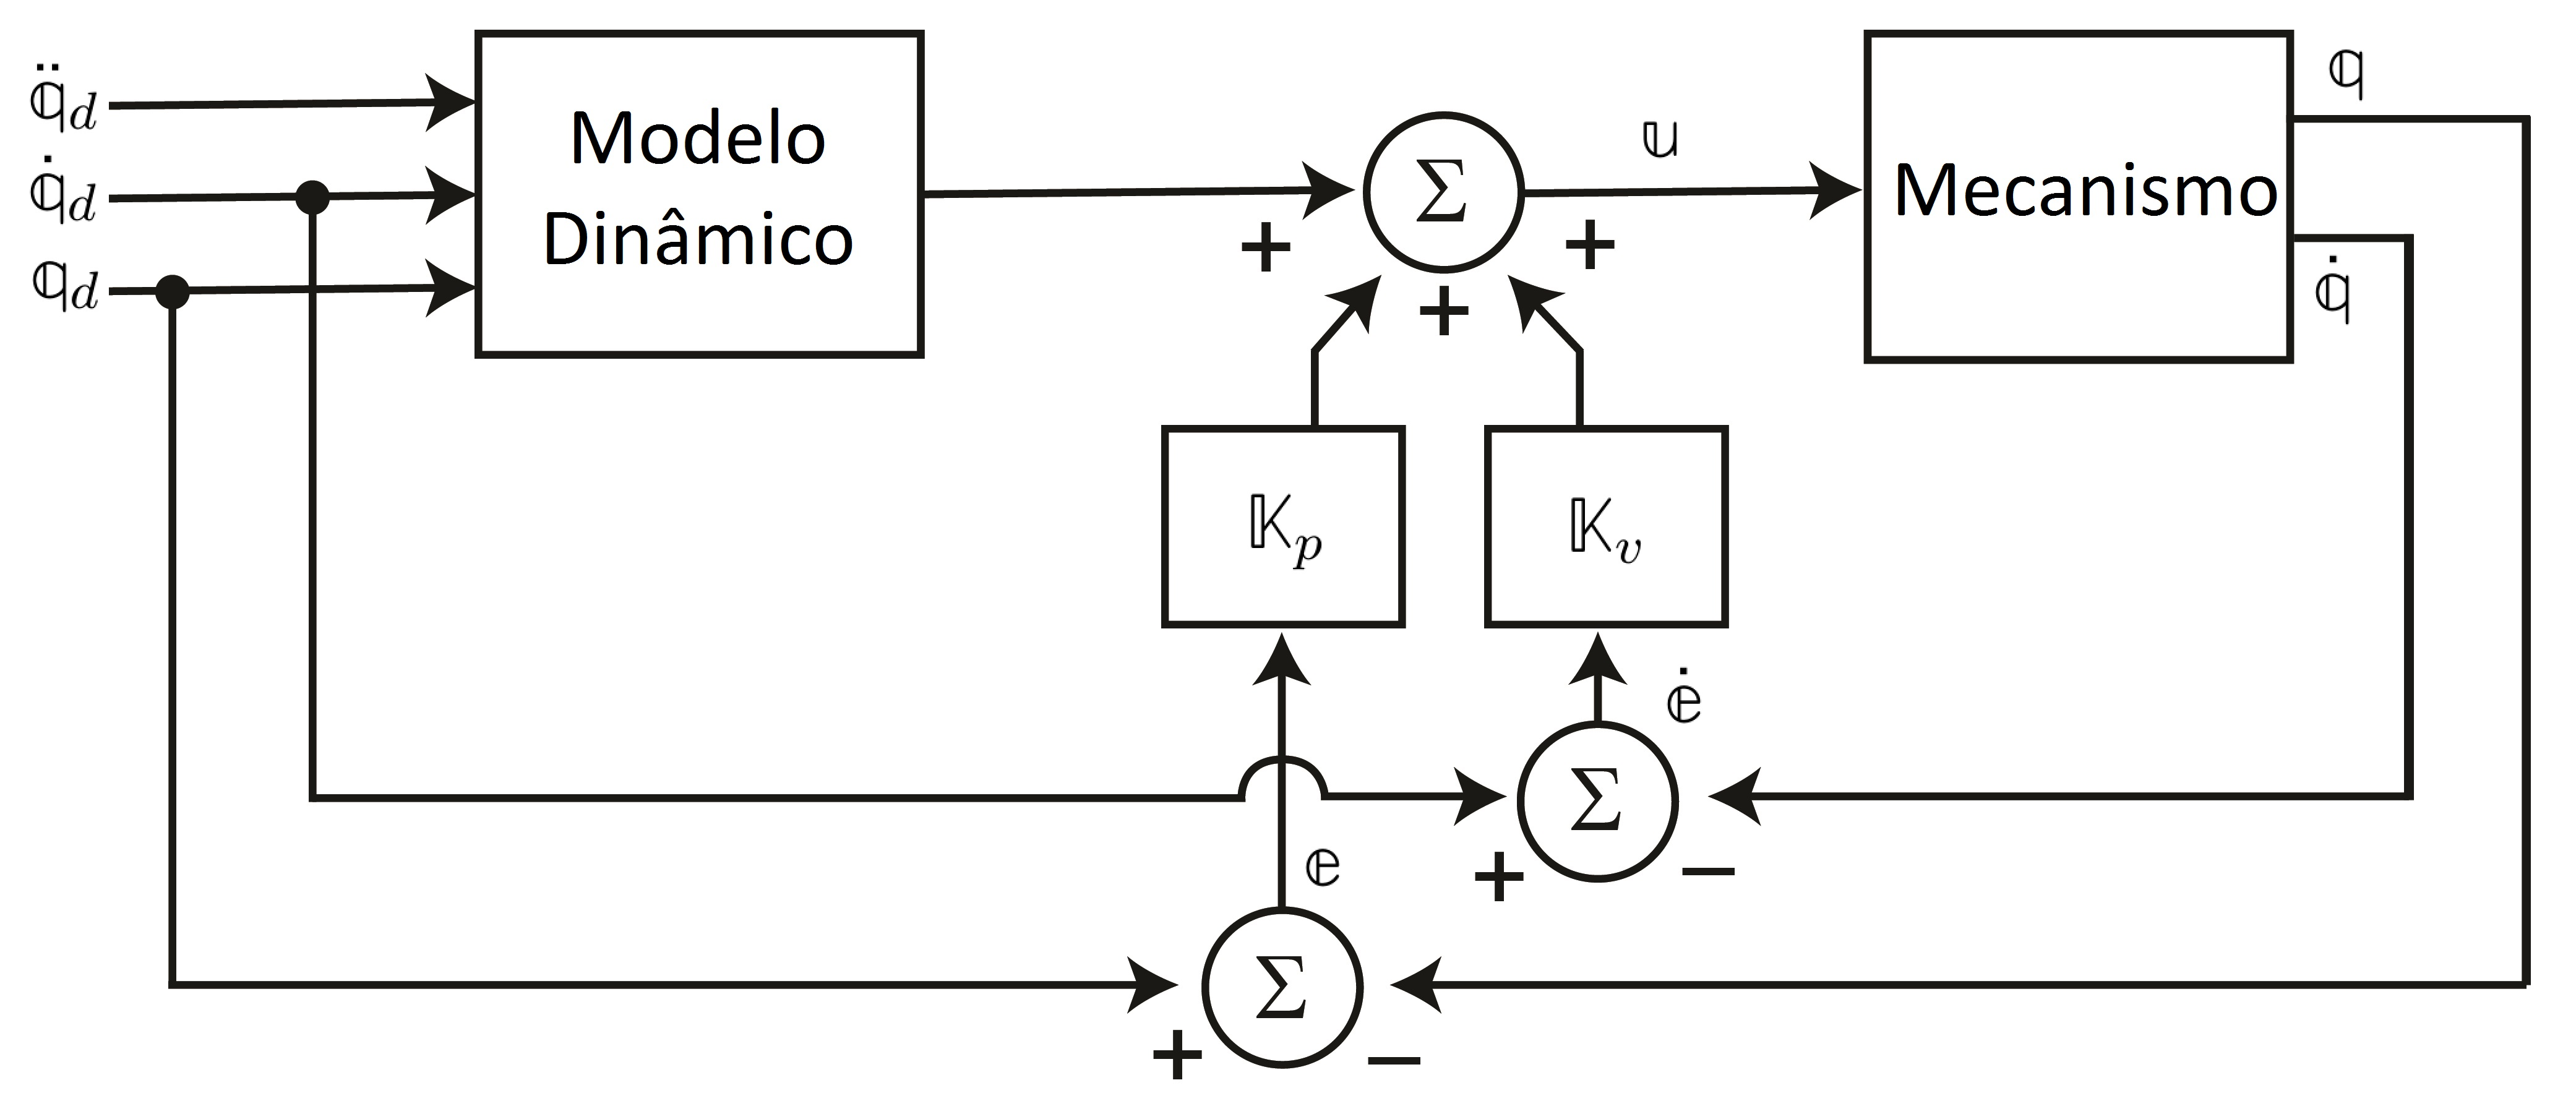
\includegraphics[scale=0.385]{../figures/CTCp.jpg}  
	\caption{Malha de CTCp (Adaptado de \cite{Craig})}
	\label{fig:CTCp}
\end{figure}

Com o intuito de melhorar a robustez do CTC associada a incertezas paramétricas, Zubizarreta et al. \cite{Zubizarreta, Zubizarreta2, Zubizarreta3, Zubizarreta4} propuseram  o  Controle por Torque Computado Estendido (CTCe), que utiliza informação redundante obtida pelo sensoriamento de juntas passivas. Em \cite{Zubizarreta}, os controladores propostos demonstraram maior robustez, principalmente em relação a parâmetros cinemáticos, durante as simulações realizadas com o mecanismo 3-RRR.

Outra técnica alternativa, aplicada a mecanismos paralelos, é o controle preditivo baseado em modelo (CPM). Para a sua implementação, o CPM necessita minimizar uma função objetivo, dependente das saidas e do esforço de controle, ambos calculados em tempo futuro \cite{Camacho}. Assim, dependendo do modelo utilizado, o processo de otimização pode agregar um custo computacional que inviabilize o controle, comprometendo a motivação inicial de aprimorar o desempenho do sistema. Como exemplos de utilização do CPM, podem ser citados os trabalhos de Vivas et al. \cite{Vivas} e   Duchaine et al. \cite{Duchaine}.

Com o propósito de controlar o mecanismo H4, Vivas et al. \cite{Vivas} utilizaram  uma malha de CPM linear e outra malha para compensação das não linearidades. Após a comparação do desempenho do controlador proposto com  o CTC, os autores observaram maior robustez do CPM a incertezas paramétricas. 

Duchaine et al. \cite{Duchaine}, por sua vez, propuseram um controlador preditivo baseado no modelo não linear de um mecanismo paralelo de 6 graus de liberdade. Visando a obtenção de uma solução analítica para o problema de otimização, foram adotadas diversas hipóteses simplificadoras no modelo dinâmico do mecanismo. Com o intuito de comparar o controlador proposto com um PID, foram feitos alguns experimentos, onde se observou  que o CPM apresentou erro nulo de posição no final da trajetória, enquanto que o PID demorou um tempo considerável para alcançar erro nulo. Foi verificada a equivalência entre o custo computacional dos 2 controladores. 

O controle adaptativo, também encontrado na literatura, caracteriza-se pela utilização de leis de adaptação para realizar a estimação em tempo real de parâmetros do sistema ou de termos de compensação dinâmica. Sendo assim, as técnicas de controle adaptativo possibilitam que o sistema se torne praticamente insensível a incertezas paramétricas. Para o caso em que se realiza a estimação em tempo real dos parâmetros do sistema, pode-se dizer que o custo computacional é superior ao do CTC, visto que é necessário integrar as leis de adaptação em tempo real. Além disso, é necessário obter o modelo dinâmico linear em relação aos parâmetros do sistema \cite{SlotiniA}, o que pode ser uma tarefa difícil, inviabilizando, em alguns casos, a aplicação da técnica. Em \cite{Codourey2} é proposto um algoritmo de obtenção do modelo dinâmico simplificado de mecanismos paralelos nesse formato.

Em \cite{SlotiniA} é proposta uma lei de controle que combina o controle adaptativo com a técnica de controle robusto conhecida por Controle por Modos Deslizantes. Chemori et al. \cite{Chemori} utilizaram essa técnica  com o intuito de diminuir os erros de posição em regime permanente no controle de um mecanismo paralelo do tipo PAR2. Por outro lado, Honegger at al. \cite{Honegger} empregaram o controle adaptativo com estimação em tempo real dos parâmetros do sistemas, realizando a compensação dinâmica por pré-alimentação, em um mecanismo  paralelo do tipo Hexaglide.

\begin{figure}[h]
	\centering
	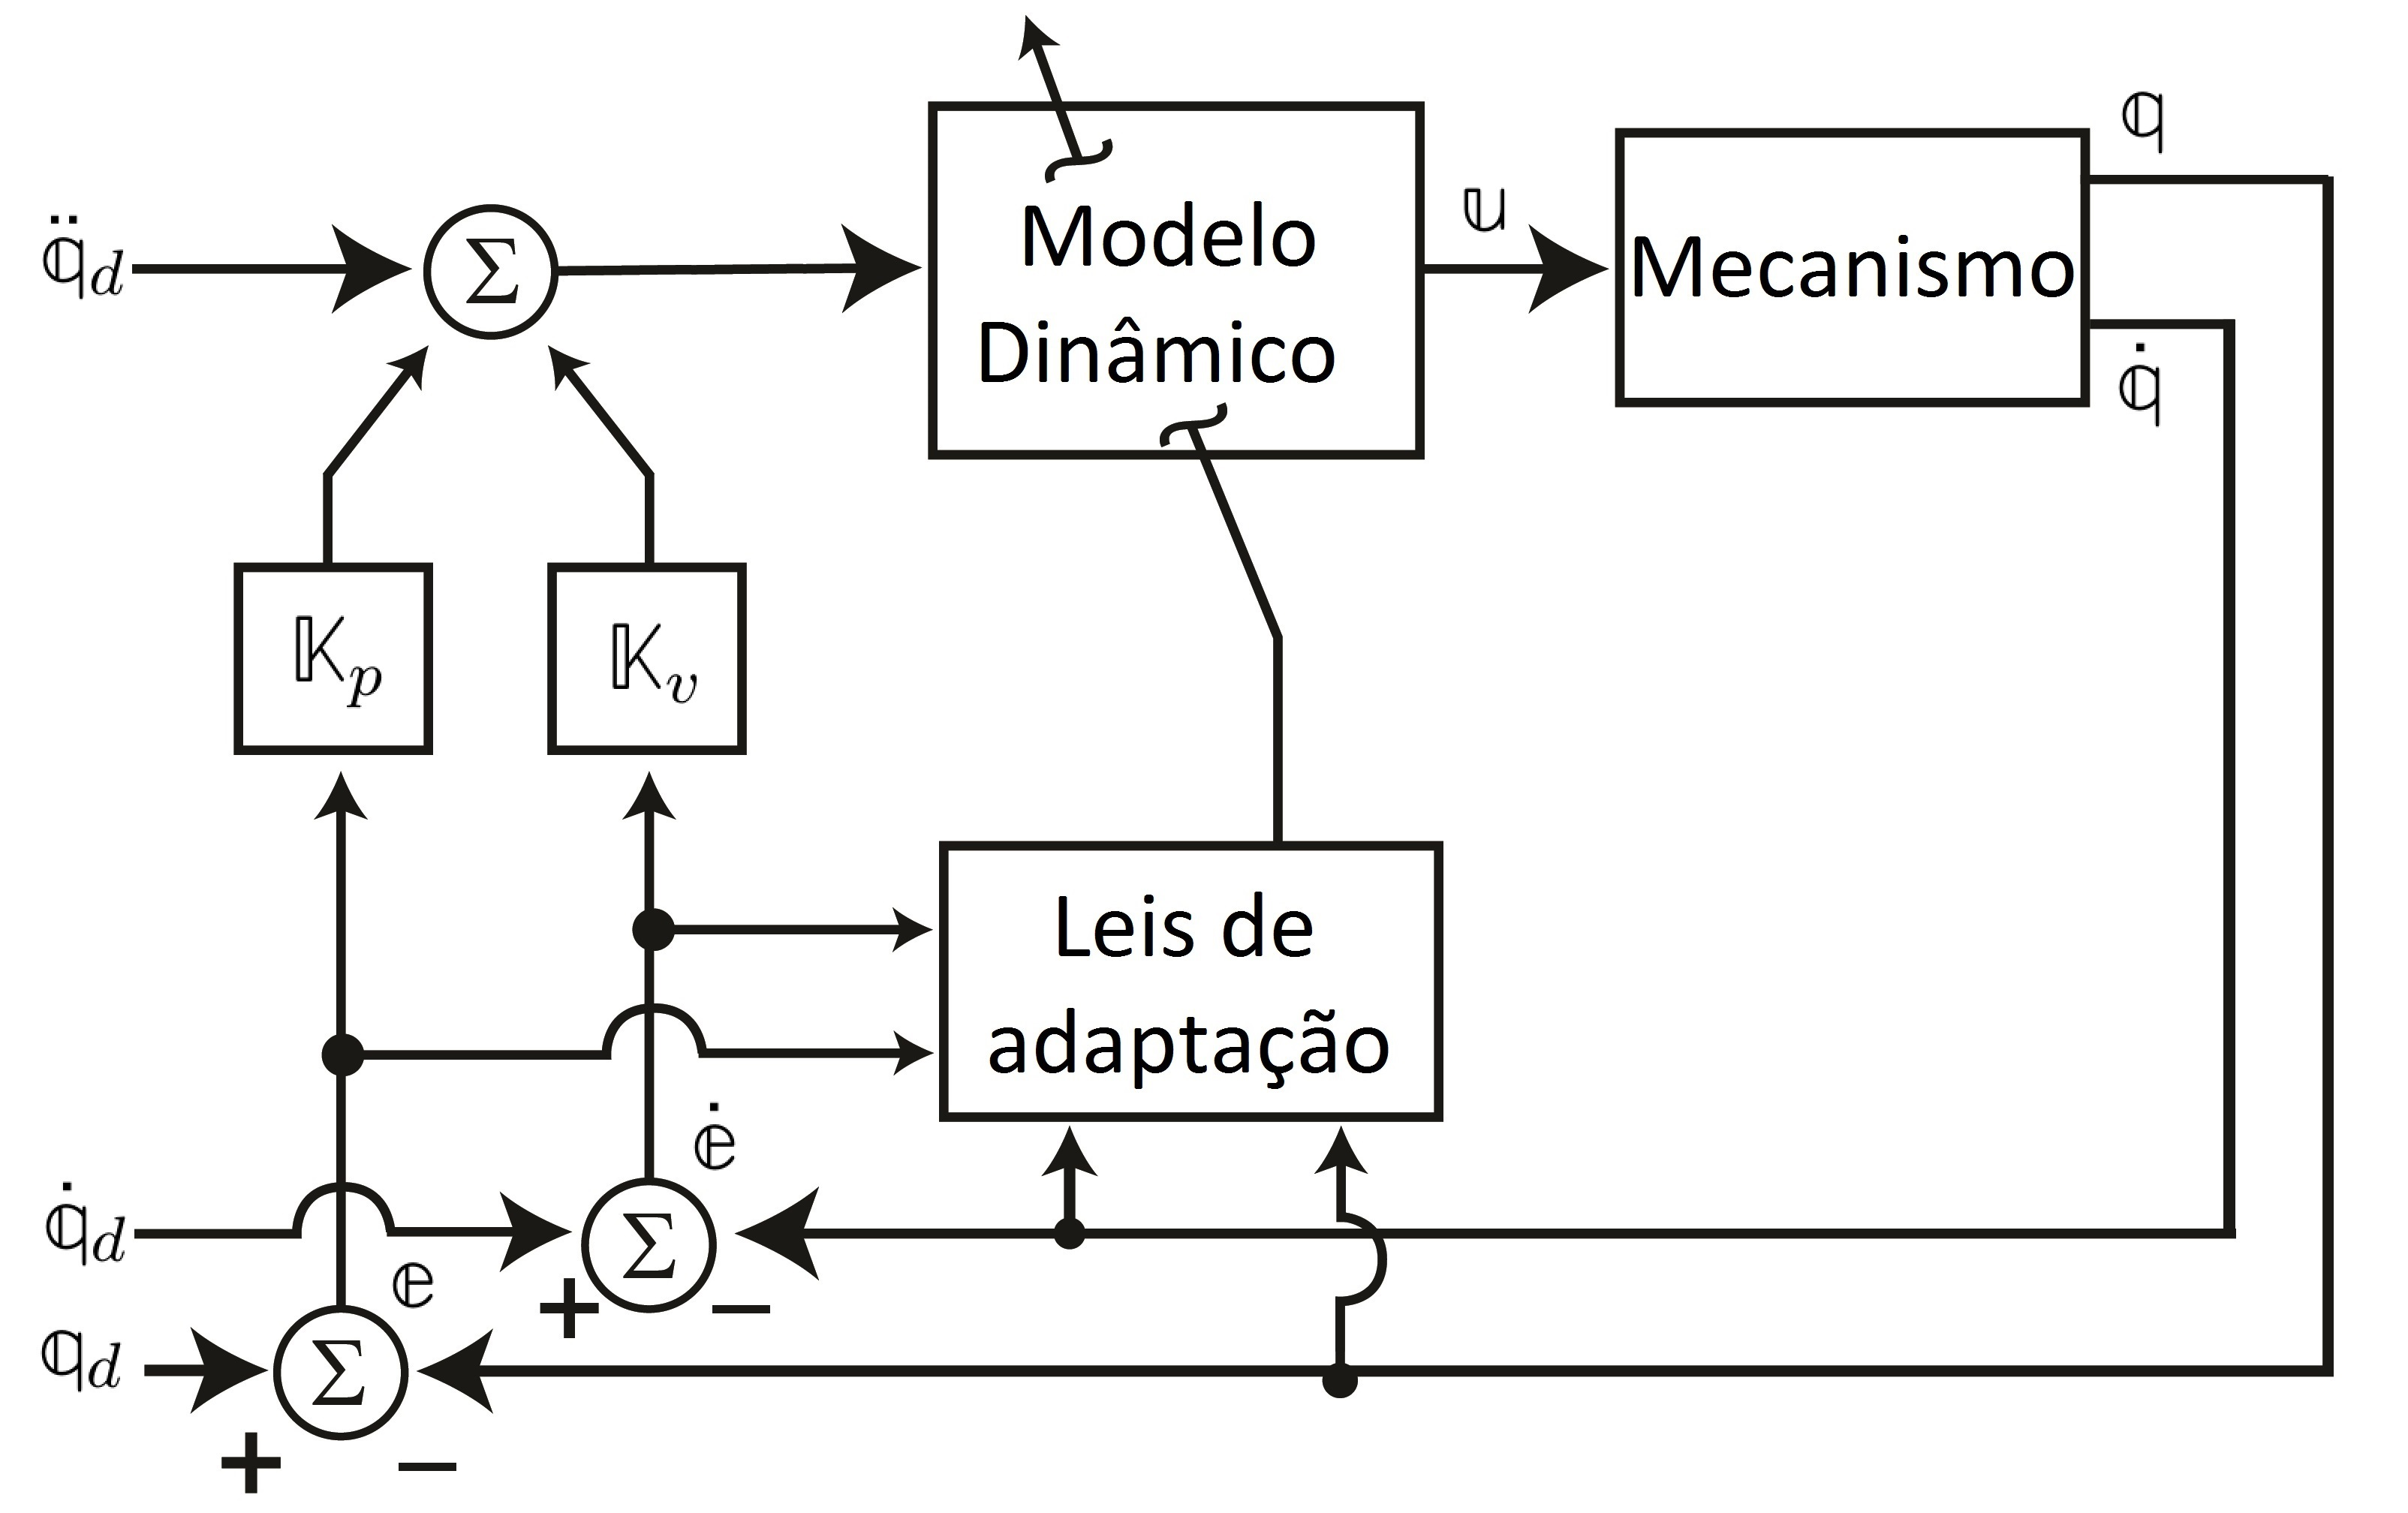
\includegraphics[scale=0.385]{../figures/CA.jpg}  
	\caption{Malha de controle adaptativo (Adaptado de \cite{Craig})}
	\label{fig:CTCp}
\end{figure}

Outra técnica promissora para aplicação em mecanismos paralelos é o Controle por Modos Deslizantes (CMD). A técnica consiste no projeto de leis de controle que levem o sistema para superfícies de escorregamento no espaço de fase, de modo que assim que o sistema atinje e é mantido nas superfícies de escorregamento, o erro de controle decai exponencialmente para zero \cite{Slotini}. Para garantir que o sistema atinja em tempo finito e se mantenha nas superfícies de escorregamento, são utilizados termos descontínuos na lei de controle, o que pode causar problemas de oscilações bruscas em alta frequência nos esforços de controle ({\em chattering}). Em \cite{Guldner}  e  \cite{Utkin2} são propostas técnicas para evitar esse tipo de problema. A grande vantagem da utilização deste tipo de lei de controle é sua grande robustez a incertezas estruturadas e não estruturadas, sendo possível realizar o projeto do controlador de modo a suprimir um dado nível de incertezas paramétricas. Em \cite{SlotiniSMC} é proposta uma metodologia de projeto de Controle por Modos Deslizantes para manipuladores robóticos seriais.

Na literatura são encontradas diversos artigos utilizando a técnica de CMD aliada à lógica {\em fuzzy} e/ou redes neurais para o controle de manipuladores robóticos \cite{Begon, Ertugrul, Hu, Sadati}. Begon et al. \cite{Begon} propuseram uma lei de controle baseada na teoria de CMD e na utilização de lógica {\em fuzzy} para controlar de maneira independente os atuadores de um mecanismo paralelo do tipo Hexa. A técnica proposta teve o intuito de obter a robustez característica do CDM sem necessitar de uma lei de controle com termos descontínuos, evitando o {\em chattering}.

Em \cite{Zeinali}, Zeinali et al. desenvolveram uma lei de controle  baseada nas teorias de CMD e controle adaptativo. O controlador desenvolvido realiza a compensação dinâmica em tempo real do erro de modelagem através de uma lei de adaptação. Além disso, substitui o termo descontínuo da lei de controle por um termo do tipo PID, com o intuito de evitar o {\em chattering}. A estabilidade e robustez da lei de controle proposta foram provadas utilizando a teoria de estabilidade de Lyapunov \cite{Slotini}. A robustez da lei de controle foi verificada através de simulações do controlador proposto aplicado a um mecanismo serial do tipo \underline{R}\underline{R}, nas quais o controlador conseguiu manter erros de posição muito pequenos em regime permanente, mesmo sendo baseado em um modelo muito pobre e na presença de distúrbios de torque. A técnica apresentada se mostra promissora, porém, como no artigo foi feita apenas a simulação da lei de controle em um mecanismo serial bidimensional, ainda não se pode afirmar nada sobre seu desempenho em mecanismos paralelos tridimensionais.

%METODOLOGIA--------------------------------------------------------------------
\chapter{Metodologia da tese}\label{method}

O estágio atual de desenvolvimento do presente projeto ocorre basicamente em três áreas:
aplicação do algoritmo de modelagem e simulação para os mecanismos 5R \cite{22orsino} e 2\underline{R}SU + \underline{P}PaP \cite{Kumazawa}, o projeto e simulação de controladores não lineares robustos de alto desempenho baseado no modelo dinâmico para os mecanismos citados, e a validação experimental das leis de controle sintetizadas.

Os trabalhos no âmbito de modelagem e simulação estão sendo desenvolvidos a partir da aplicação do algoritmo de modelagem cinemática e dinâmica de mecanismos paralelos desenvolvido, baseado na utilização dos parâmetros de Denavit-Hartenberg \cite{Craig, Denavit, Lipkin} e no método Orsino de acoplamento de subsistemas \cite{23orsino}. Toda modelagem será feita em C++, utilizando uma biblioteca otimizada de cálculo matricial (Armadillo).
As simulações da dinâmica direta do mecanismo serão feitas utilizando o método Runge-Kutta de 8ª ordem \cite{RK} para solução de sistemas de EDOs, de modo a garantir estabilidade numérica do método, mesmo utilizando leis de controle quase descontínuas.

Os trabalhos na área de projeto de controle serão feitos utilizando a metodologia desenvolvida de projeto de controladores robustos multivariáveis para mecanismos paralelos, baseada no modelo dinâmico do mecanismo a ser controlado e na técnica de controle por modos deslizantes \cite{Slotini, Utkin}.

Os trabalhos no âmbito da validação experimental das leis de controle sintetizadas serão realizados no protótipo do mecanismo 5R que encontra-se no laboratório de mecanismos. A bancada experimental do mecanismo 5R já está funcional e já forem realizados alguns testes de leis de controle de trajetória baseadas no modelo dinâmico do mecanismo. Para a realização da validação experimental nesta bancada, será realizada a identificação dos parâmetros do sistema e suas respectivas incertezas, projeto do controlador baseado nos parâmetros e incertezas identificadas, implementação das leis de controle, e aquisição de dados. \\

\begin{figure}[h!]
	\centering
	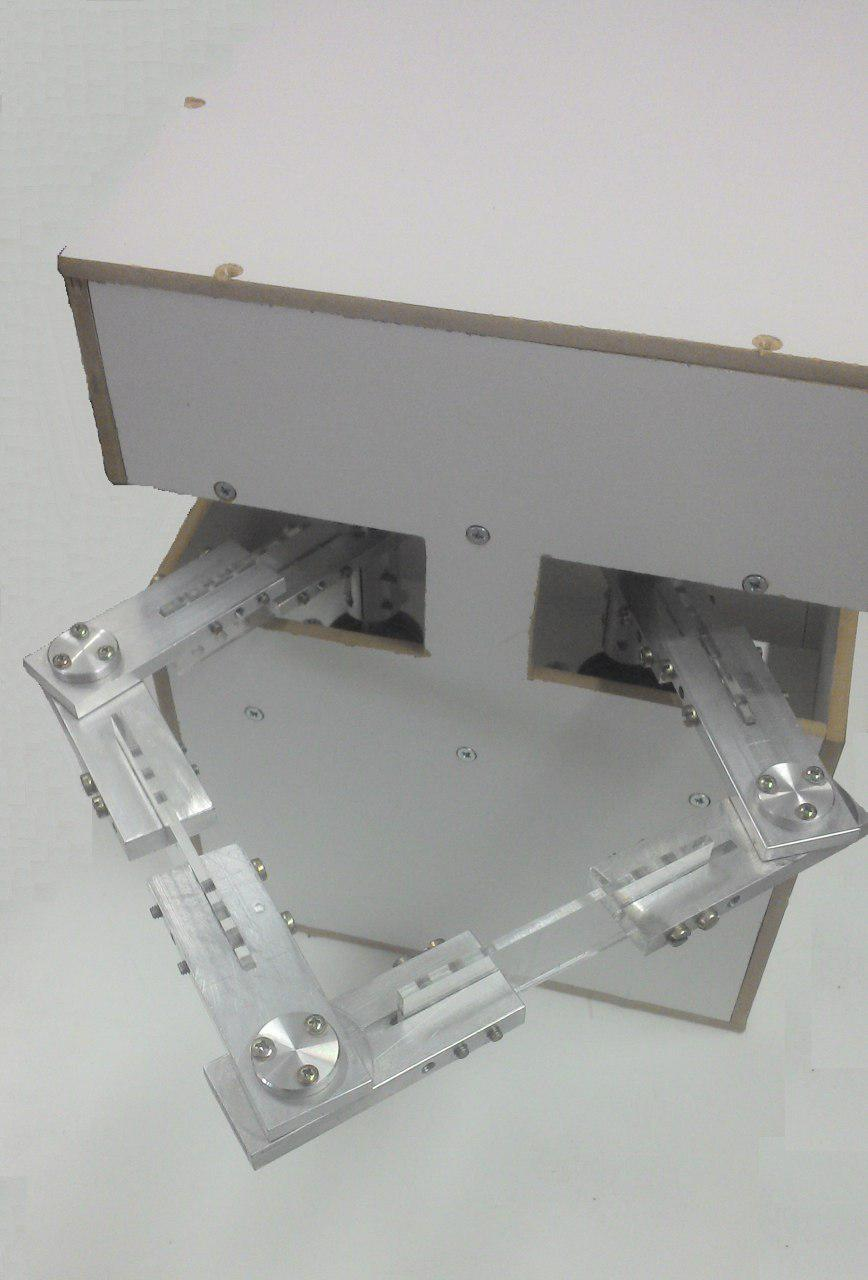
\includegraphics[scale=0.3]{../figures/Clara.jpg}  
	\caption{Protótipo do mecanismo 5R}
	\label{fig:Mecanismo2}
\end{figure}

\blinddocument


% ========== Referências ==========
% --- IEEE ---
%	http://www.ctan.org/tex-archive/macros/latex/contrib/IEEEtran
%\bibliographystyle{IEEEbib}

% --- ABNT (requer ABNTeX 2) ---
%	http://www.ctan.org/tex-archive/macros/latex/contrib/abntex2
%\bibliographystyle{abntex2-num}

%\bibliography{}


% ========== Apêndices (opcional) ==========
\apendice
\chapter{}
\chapter{Beta}


% ========== Anexos (opcional) ==========
\anexo
\chapter{Alpha}
\chapter{}



\end{document}
